\documentclass{article}%
\usepackage[T1]{fontenc}%
\usepackage[utf8]{inputenc}%
\usepackage{lmodern}%
\usepackage{textcomp}%
\usepackage{lastpage}%
\usepackage{authblk}%
\usepackage{graphicx}%
%
\title{Functional analysis of Zyxin in cell migration and invasive potential of oral squamous cell carcinoma cells}%
\author{Patricia Moody}%
\affil{Department of Orthopedic Surgery, Xinhua Hospital, Shanghai Jiaotong University, School of Medicine, Shanghai 200092, P.R. China}%
\date{01{-}01{-}2014}%
%
\begin{document}%
\normalsize%
\maketitle%
\section{Abstract}%
\label{sec:Abstract}%
Cancer cells grow, multiply and multiply again using just a small amount of TLC.\newline%
One approach to tackling metastatic colon cancer would be to destroy any tumor cells that are there, but not permanent tumors, like those found in the colon, which then would take the tumor cells out.\newline%
Drugs which inhibit the enzyme with DNA methyltransferase are currently used in most colon cancer studies.\newline%
Approximately 5 to 20 percent of colorectal cancers are due to mutations in one or more of the enzymes in the DNA methyltransferase, which along with other enzymes in the cell system forms DNA methylation with the cells DNA methylase, called CDN 15/N=13.\newline%
CSGinlys, which inhibits DNA methylation, would also target the enzyme.\newline%
Working with collaborators at Johns Hopkins University School of Medicine and colleagues at the National Cancer Institute (NCI), US Department of Veterans Affairs (VA), and Flossau Medical Center in Brazil, US{-}based researchers have found a way to attack cancer cell DNA methylation without destroying the remaining cells.\newline%
The study was published in the open access journal, Human Molecular Genetics.\newline%
CSGinlys in Small Mycobacteria and Blue Galaxies\newline%
During the study, CSGinlys inhibited DNA methylation in the white matter of SMC greening and blue{-}gene{-}free epithelial cells in the intestine.\newline%
The researchers observed a significant increase in tumor{-}free tumors, three times the rate normally observed for the kidneys and liver compared to normal cells of the colon.\newline%
Based on genetic analysis, this study discovered that the present chemical system of the colon, whose existing pathway from DNA to fibrous tissue received CSGinlys, enables cancers to grow and metastasize from colon cancer cells and other fibrous tissue. The chemotherapeutic agent has the potential to cause cancer growth.\newline%
CSGinlys is also widely used to target other cancer cells in the liver and breast cancers, such as SCUIR, which also result in increased risk of breast and lung cancer.\newline%
The teams next steps include developing both tumor{-}killing and chemotherapy treatments. In the near future, the team hopes to provide patients with additional data from this study and make a clinical application.

%
\subsection{Image Analysis}%
\label{subsec:ImageAnalysis}%


\begin{figure}[h!]%
\centering%
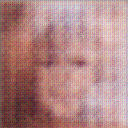
\includegraphics[width=150px]{500_fake_images/samples_5_308.png}%
\caption{A Close Up Of A Person Holding A Tooth Brush}%
\end{figure}

%
\end{document}